\documentclass[a4paper, 14pt]{extarticle}
\usepackage[utf8]{inputenc}
\usepackage[paper=a4paper, top=1cm, right=1cm, bottom=1.5cm, left=2cm]{geometry}
\usepackage{setspace}
\onehalfspacing

\usepackage{graphicx}
\graphicspath{{plots/}, {images/}}

\parindent=1.25cm

\usepackage{titlesec}

\titleformat{\section}
    {\normalsize\bfseries}
    {\thesection}
    {1em}{}

\titleformat{\subsection}
    {\normalsize\bfseries}
    {\thesubsection}
    {1em}{}

% Настройка вертикальных и горизонтальных отступов
\titlespacing*{\chapter}{0pt}{-30pt}{8pt}
\titlespacing*{\section}{\parindent}{*4}{*4}
\titlespacing*{\subsection}{\parindent}{*4}{*4}

\usepackage[square, numbers, sort&compress]{natbib}
\makeatletter
\bibliographystyle{unsrt}
\renewcommand{\@biblabel}[1]{#1.} 
\makeatother


\newcommand{\maketitlepage}[6]{
    \begin{titlepage}
        \singlespacing
        \newpage
        \begin{center}
            Министерство образования и науки Российской Федерации \\
            Федеральное государственное бюджетное образовательное \\
            учреждение высшего профессионального образования \\
            <<Волгоградский государственный технический университет>> \\
            #1 \\
            Кафедра #2
        \end{center}


        \vspace{14em}

        \begin{center}
            \large Семестровая работа #6 по дисциплине
            \\ <<#3>>
        \end{center}

        \vspace{5em}

        \begin{flushright}
            \begin{minipage}{.35\textwidth}
                Выполнила:\\#4
                \vspace{1em}\\
                Проверил:\\#5
                \\
                \\ Оценка \underline{\ \ \ \ \ \ \ \ \ \ \ \ \ \ \ \ }
            \end{minipage}
        \end{flushright}

        \vspace{\fill}

        \begin{center}
            Волгоград, \the\year
        \end{center}

    \end{titlepage}
    \setcounter{page}{2}
}

\newcommand{\maketitlepagewithvariant}[7]{
    \begin{titlepage}
        \singlespacing
        \newpage

        \begin{center}
            Министерство образования и науки Российской Федерации \\
            Федеральное государственное бюджетное образовательное \\
            учреждение высшего профессионального образования \\
            <<Волгоградский государственный технический университет>> \\
            #1 \\
            Кафедра #2
        \end{center}


        \vspace{8em}

        \begin{center}
            \large Семестровая работа #6 по дисциплине
            \\ <<#3>>
        \end{center}

        \vspace{1em}
        \begin{center}
            Вариант №#7
        \end{center}
        \vspace{4em}

        \begin{flushright}
            \begin{minipage}{.35\textwidth}
                Выполнила:\\#4
                \vspace{1em}\\
                Проверил:\\#5
                \\
                \\ Оценка \underline{\ \ \ \ \ \ \ \ \ \ \ \ \ \ \ \ }
            \end{minipage}
        \end{flushright}

        \vspace{\fill}

        \begin{center}
            Волгоград, \the\year
        \end{center}

    \end{titlepage}
    \setcounter{page}{2}
}

\input{../.preambles/10-russian}
\input{../.preambles/20-math}
\input{../.preambles/30-physics}
\begin{document}
\maketitlepage{Факультет электроники и вычислительной техники}{физики}
{Электродинамика}{студент группы Ф-369\\Чечеткин~И.~А.}
{доцент Грецов~М.~В.}{№1}
\emph{83.} Заряд электрона распределен в атоме водорода, находящемся в
нормальном состоянии, с плотностью
\[
  \rho(r) = -\frac{e_0}{\pi a^3}e^{-\frac{2r}{a}},
\]
где \( a = 0,529\cdot10^{-8} \)~см -- боровский радиус электрона,
\( e_0 = 4,80\cdot10^{-10} \)~CGSE -- элементарный заряд. Найти потенциал
\( \phi_e \) и напряженность \( E_{er} \) электрического поля электронного заряда,
а также полные потенциал \( \phi \) и напряженность поля \( \vec{E} \) в атоме,
считая, что протонный заряд сосредоточен в начале координат. Построить
приблизительный ход величин \( \phi \) и \( E \).

\vspace*{2em}
\emph{Решение:}
    
    Из теоремы Гаусса:
    \[
        E_{er}(r) = \frac{1}{\Ezero r^2} \int\limits_0^r \rho(r'){r'}^2\d r'.
    \]
    
    Потенциал точечного заряда на бесконечности стремится к нулю, поэтому
    \[
        \phi_e(r) = \int\limits_r^\infty \frac{1}{\Ezero r^2}\int\limits_0^r \rho(r')
        {r'}^2\d r' = -\frac{1}{\Ezero}\int\limits_r^\infty \d\left(\frac{1}{r}
        \right)\int\limits_0^r \rho(r'){r'}^2\d r'.
    \]
    Взяв интеграл по частям, получим:
    \[
        \phi_e(r) = \frac{1}{\Ezero r}\int\limits_0^r \rho(r'){r'}^2\d r' +
        \frac{1}{\Ezero}\int\limits_r^\infty \rho(r')r'\d r'.
    \]
    
    Подставляя плотность распределения заряда \( \rho \) в формулы для
    \( E_{er}(r) \) и \( \phi_r(r) \), получим:
    \begin{align*}
        & \phi_e(r) = \frac{e_0}{r}\left[e^{-\frac{2r}{a}} - 1\right] +
        \frac{e_0}{a}e^{-\frac{2r}{a}}, \\
        & E_{er}(r) = \frac{e_0}{r^2}\left[\left(1 + \frac{2r}{a}\right)
        e^{-\frac{2r}{a}} - 1\right] + \frac{2e_0}{a^2}e^{-\frac{2r}{a}}.
    \end{align*}
    
    Воспользовавшись принципом суперпозиции, найдем потенциал \( \phi(r) \) и
    напряженность поля \( E(r) \) в атоме:
    \begin{align*}
        & \phi(r) = \phi_e(r) + \phi_\emph{п}(r) = \phi_e(r) + \frac{e_0}{r} =
        e_0e^{-\frac{2r}{a}}\left[\frac{1}{r} + \frac{1}{a}\right], \\
        & E(r) = E_{er}(r) + E_\emph{п}(r) = E_{er}(r) + \frac{e_0}{r^2} =
        e_0e^{-\frac{2r}{a}}\left[\frac{1}{r^2} + \frac{2}{ar} + \frac{2}{a^2}
        \right].
    \end{align*}
    
    \begin{figure}
        \center
        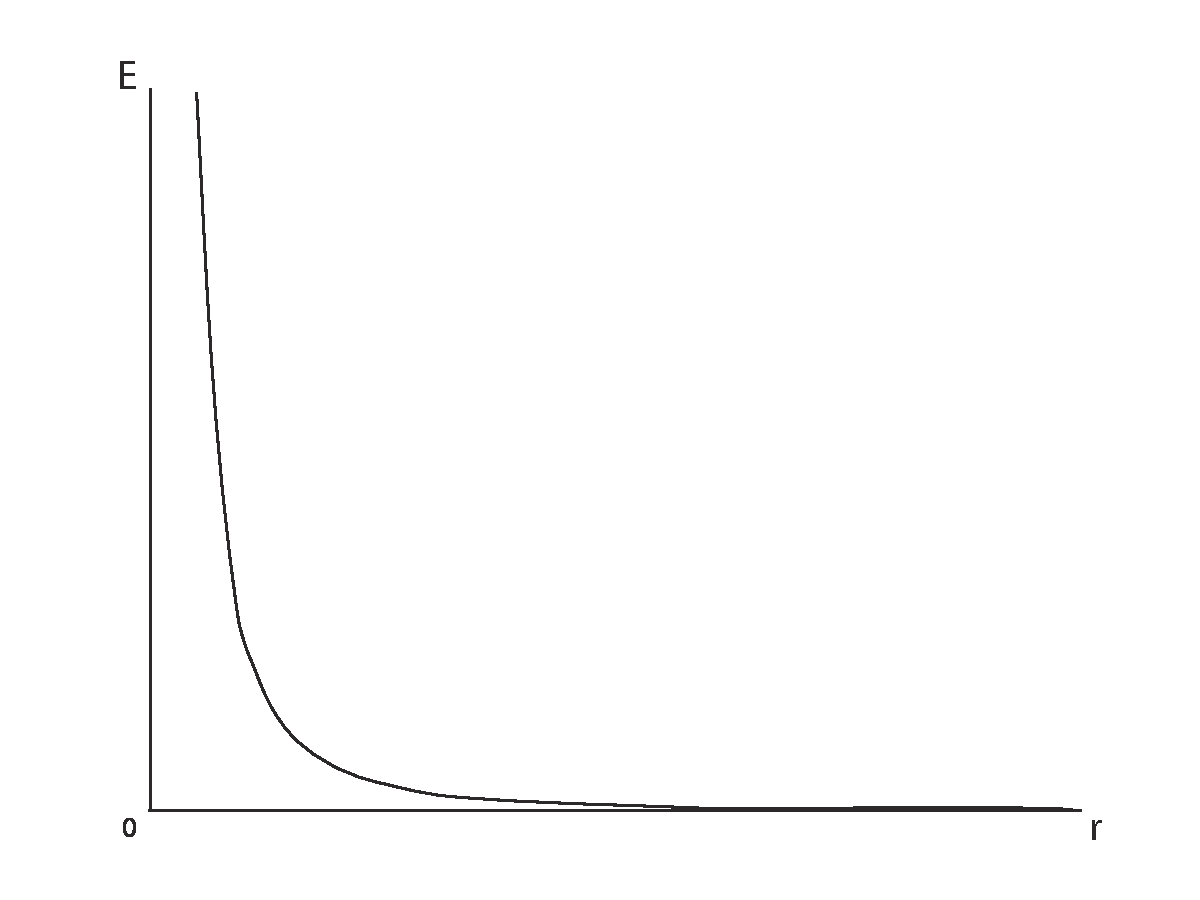
\includegraphics[width=.47\textwidth]{field}\hfill
        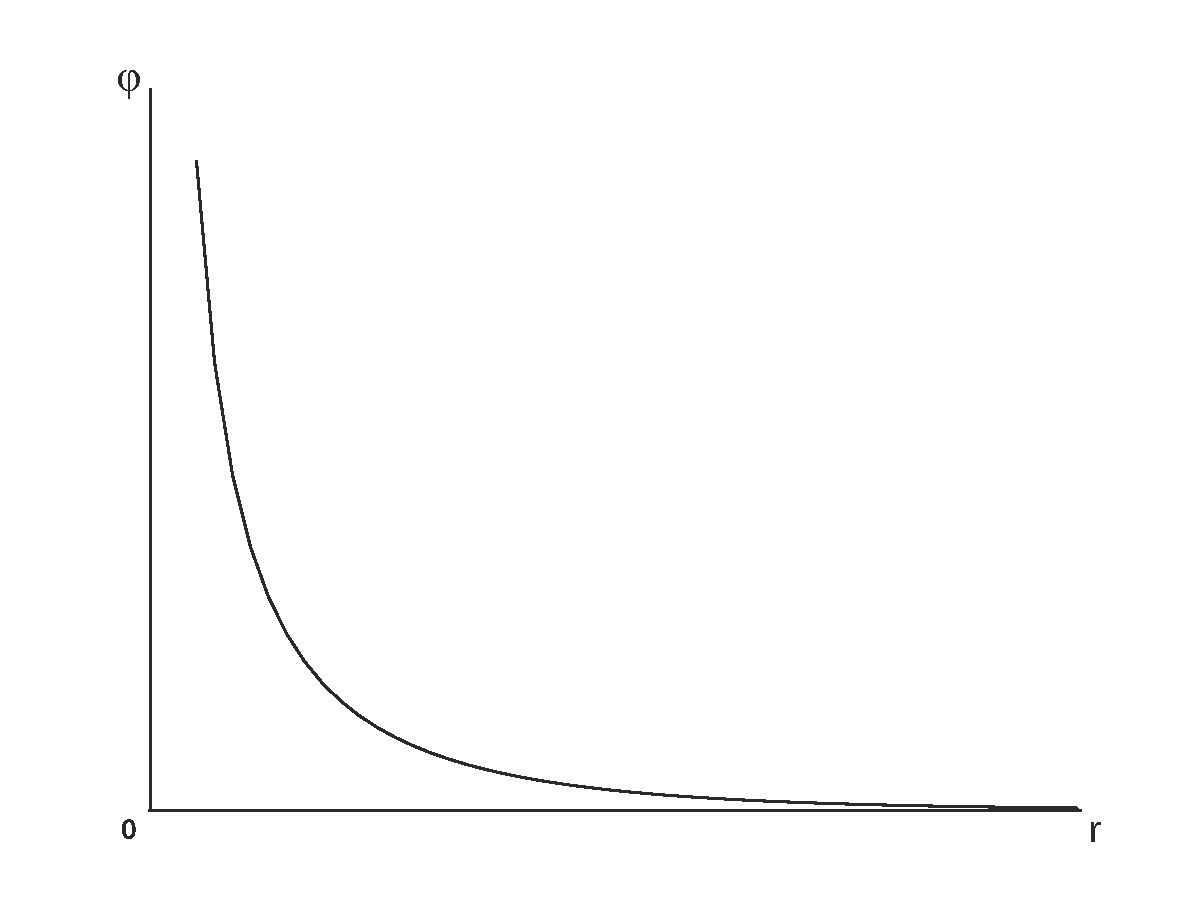
\includegraphics[width=.47\textwidth]{potential}
        \parbox{.47\textwidth}{\centering Зависимость \( E(r) \)}\hfill
        \parbox{.47\textwidth}{\centering Зависимость \( \phi(r) \)}
    \end{figure}

\vspace*{2em}        
\emph{Ответ:}
    \begin{align*}
        & \phi_e(r) = \frac{e_0}{r}\left[e^{-\frac{2r}{a}} - 1\right] +
        \frac{e_0}{a}e^{-\frac{2r}{a}}, \\
        & E_{er}(r) = \frac{e_0}{r^2}\left[\left(1 + \frac{2r}{a}\right)
        e^{-\frac{2r}{a}} - 1\right] + \frac{2e_0}{a^2}e^{-\frac{2r}{a}}; \\
        & \phi(r) = e_0e^{-\frac{2r}{a}}\left[\frac{1}{r} + \frac{1}{a}\right], \\
        & E(r) = e_0e^{-\frac{2r}{a}}\left[\frac{1}{r^2} + \frac{2}{ar} +
        \frac{2}{a^2}\right].
    \end{align*}
\newpage
%-------------------------------------------------------------------------------
\emph{253.} Сфера радиуса \( a \) заряжена зарядом \( e \) равномерно по
поверхности и вращается вокруг одного из своих диаметров с угловой скоростью
\( \vec{\omega} \). Найти магнитное поле внутри и вне сферы. Выразить
напряженность поля \( \vec{H} \) во внешней области через магнитный момент
\( \vec{m} \) сферы.

\vspace*{2em}
\emph{Решение:}
\vfill
\emph{Ответ:}
\newpage
%-------------------------------------------------------------------------------
\emph{548.} Пусть для измерения времени используется периодический процесс
отражения светового <<зайчика>> попеременно от двух зеркал, укрепленных на
концах стержня длиной \( l \). Один период -- это время движения <<зайчика>> от
одного зеркала до другого и обратно. Световые часы неподвижны в системе \( S' \)
и ориентированы перпендикулярно направлению относительной скорости.
Пользуясь постулатом о постоянстве скорости света, показать, что интервал
собственного времени \( \d\tau \) выражается через промежуток времени \( \d t \)
в системе \( S \).

\vspace*{2em}
\emph{Решение:}
    
    В системе \( S' \) имеем:
    \[
        c\d\tau = 2l.
    \]
    
    В системе \( S \):
    \[
        c\d t = 2\sqrt{l^2 + \left(\frac{v\d t}{2}\right)^2}.
    \]
    
    Возводя последнее равенство в квадрат и перенося \( v^2\d t^2 \) в левую часть,
    получим
    \[
        \d t^2c^2\left[1 - \left(\frac{v}{c}\right)^2\right] = 4l^2.
    \]
    
    Разделив полученное выражение на \( c^2 \) и извлекая квадратный корень,
    получим:
    \[
        \d\tau = \frac{2l}{c} = \d t\sqrt{1 - \left(\frac{v}{c}\right)^2}.
    \]
    
\vfill
\emph{Ответ:}
    \[
        \d\tau = \frac{2l}{c} = \d t\sqrt{1 - \left(\frac{v}{c}\right)^2}.
    \]
\end{document}
